\documentclass[conference]{IEEEtran}
\IEEEoverridecommandlockouts
% The preceding line is only needed to identify funding in the first footnote. If that is unneeded, please comment it out.
\usepackage{cite}
\usepackage{amsmath,amssymb,amsfonts}
\usepackage{algorithmic}
\usepackage{graphicx}
\usepackage{textcomp}
\usepackage{xcolor}
\usepackage{cite}\usepackage[latin1]{inputenc}
\usepackage{tikz}
\usepackage{subcaption}
\usepackage{tabularx}
\usepackage{url}
\usepackage{nicefrac}
\usetikzlibrary{positioning}
\usetikzlibrary{shapes,arrows}


%COMMANDS
\newcommand{\argmax}{\mathop{\mathrm{argmax}}\limits}
\newcommand{\xf}{\mathbf{x}}
\newcommand{\yf}{\mathbf{y}}
\newcommand{\zf}{\mathbf{z}}
\newcommand{\pf}{\mathbf{p}}


\newcommand{\yfh}{\hat{\mathbf{y}}}


\def\BibTeX{{\rm B\kern-.05em{\sc i\kern-.025em b}\kern-.08em
    T\kern-.1667em\lower.7ex\hbox{E}\kern-.125emX}}

\bibliographystyle{bst2aurth}
\begin{document}

\title{AAnchor: CNN guided detection of anchor amino acids in high resolution cryo-EM density maps \\
%{\footnotesize \textsuperscript{*}Note: Sub-titles are not captured in Xplore and
%should not be used}
\thanks{This work has been supported in part by Len Blavatnik and the Blavatnik
Family Foundation and by the ICORE program of the Budgeting and Planning
Committee and Israel Science Foundation. M.R. was supported in part by a Ph.D. fellowship from the Edmond J. Safra Center for Bioinformatics at Tel Aviv University.}
}
\author{\IEEEauthorblockN{Mark Rozanov}
\IEEEauthorblockA{\textit{Blavatnik School of Computer Science} \\
\textit{Tel Aviv University}, 
Israel \\
markroza@tau.ac.il}
\and
\IEEEauthorblockN{Haim J. Wolfson}
\IEEEauthorblockA{\textit{Blavatnik School of Computer Science} \\
\textit{Tel Aviv University}, 
Israel \\
wolfson@tau.ac.il}
}
%\tableofcontents
\newpage
\maketitle
\pagenumbering{arabic}

%\onecolumn
%\Large

Marik Privet

\begin{abstract}
The recent cryo-EM resolution revolution enables the development of algorithms for 
direct de-novo modeling of protein structures into cryo-EM density maps. 
Here we present a machine learning based method for the detection of 
high confidence anchor amino acid residues in such a map. Such anchor residues
can be exploited in several local de-novo modeling tasks, such as the reliable positioning of secondary
structures, loop modeling and general fragment based modeling.
In the experimental results we show the ability of the proposed procedure
to locate and classify a significant number of amino acids in 
density maps of $3.1 \AA$ (or better) resolution. 
Our performance analysis indicates that the main factor affecting the detection accuracy is the 
lack of sufficient experimental data for the training stage of the algorithm.
Thus, our method is expected to improve significantly in the near future, due to the 
rapid increase in the release of novel high resolution cryo-EM maps.
\end{abstract}

\begin{IEEEkeywords}
cryo-EM maps, proteins, molecular modeling, machine learning, CNN.
\end{IEEEkeywords}
\section{Introduction}
Atomic accuracy models of protein structures are an invaluable tool for the elucidation of protein function.  The recent "resolution revolution" \cite{Kuhlbrandt2014} in cryo electron microscopy (cryoEM) has led to an ever increasing number of near atomic resolution density maps deposited in the EM databank EMDB \cite{Lawson2016}.  While in 2002 the best structure deposited was at $9 \AA$ resolution, recently (\cite{Bartesaghi2015, Banerjee2016}) key structures have been resolved at resolution better than $2.5 \AA$ .

Most of the techniques for modeling protein structures into intermediate resolution ($5 - 10 \;\AA$) maps are based on rigid fitting of template protein structures into these maps.  Many of these methods (\cite{Jiang2001,Dror2007,Yu2008,Rusu2012,Si2012}) use secondary structures as anchors for their fitting procedure. 

At resolutions better than $4-5 \AA$, the goal is more ambitious and de novo modeling techniques are being exploited. Some of them are adaptations of the standard X-ray crystallography modeling methods, however these tend to be time consuming. Recently, several de-novo modeling techniques have been developed to deal specifically with cryoEM density maps\cite{DiMaio2016}.  Pathwalking \cite{Chen2016} detects first pseudo-atom anchors and then applies the travelling salesperson (TSP) combinatorial optimization algorithm to detect a long enough path which should model the protein backbone. 
MAINMAST \cite{Terashi2018} detects a set of anchor points and calculates the backbone by applying  a minimun spanning tree (MST) approach.
A recently published method \cite{Wang2015}  fits short sequence based structure fragment templates into the density map and applies a Monte Carlo simulated annealing procedure to detect a set of mutually compatible fragments.  All of the above mentioned procedures require prior segmentation of the density map into its various protein chains.

Prior detection of reliable {\bf amino acid anchors} in the density map, namely having knowledge of even a relatively small number of amino acids, whose identity and location has been established with high confidence 
can be used to guide the various de-novo modeling methods, as well as serve as a starting point for the development of novel methods. In particular, it could lead to the development of novel techniques, which do not require prior segmentation of the EM density map.   While in high resolution maps (roughly, $3.5 \;\AA$ or better), sidechains become  visible and individual rotamers may be distinguished (\cite{DiMaio2016},\cite{Cassidy2018}), no automated method has been suggested to detect specific amino acids in a cryo-EM density map.

In this work we present a machine learning (ML) algorithm nicknamed {\bf AAnchor} (amino-acid anchor) for the detection and localization of amino acids in a high resolution cryo EM density map. 
The two primary goals of this study are 
(i) to develop an automatic tool for the detection and classification of amino acids in a near atomic resolution cryo EM map; and 
(ii) to provide a quantitative analysis of the ability to detect a specific amino acid in an experimental cryo EM map.


The preliminary results of our algorithm are quite encouraging.
For example, on the $3.1 \AA$ cryo EM map of lysenin pore \cite{Bokori-Brown2016}, the algorithm localizes above one hundred amino acids of different types with confidence above $80 \%$.
These preliminary results also indicate that the quality of detection is best for amino acids, which have a small number of rotamers and a large enough training set.  This last observation also explains why
contrary to expectation the results for  $2.9  \AA$ and $3.1 \;\AA$ resolution maps are better then those for $2.2 \;\AA$ maps. This is due to the limited training data set existing for the better resolution maps.  Thus, with the rapid increase in high resolution cryoEM structures and the availability of larger trainng sets, the results of our machine learning based methodology are expected to improve significantly.

A server of the detection/prediction stage of the  AAnchor algorithm is available at \url{http://bioinfo3d.cs.tau.ac.il/AAnchor/}.  











\section{Methods}
\subsection{The Task}
Given an electron density map of a protein/macromolecular assembly, our task is to detect voxels in this map, which correspond to the location of the centers of mass of specific amino acids.
The goal is to report only those amino acids, which have been detected with high confidence, which we call "anchors".
The two main building blocks of our method are a \textbf{classification} CNN and a \textbf{detection} algorithm.
The detection algorithm generates candidates for the classification CNN and filters out candidates of expected low accuracy. 

\subsection{A CNN for the classification task}
Convolutional neural networks (CNN) were proposed by Yann LeCun in 1989 for zip code recognition \cite[]{Y.LeCunB.BoserJ.S.DenkerD.HendersonR.E.Howard1989}.
A CNN consists of alternating convolutional and pooling layers optionally followed by fully connected layers.
The first and last layers are  the input and  output layer respectively, while the other layers are referred to as hidden layers.

Formally, a CNN of depth $D$  is a composition of $D$  parametrized functions $\{f_1,\cdots,f_D\}$, which maps an input vector $\xf$ to an output vector $\yf$:
\begin{equation}\label{cnn1}
	\yf = f(\xf) = f_D(\zf,w_D,b_D) \circ, \ldots, \circ f_1(\xf,w_1,b_1),
\end{equation}
where $w_k$ and $b_k$ are the weights and biases vectors for the function $f_k$.  The functions $f_k$ are the previously mentioned layers.

Given a set of labeled data pairs $\{(\xf^i,\yf^i)\}_{i=1}^M$, the training process of a CNN defined by \eqref{cnn1} is a process of a numerical solution of the optimization problem:
\begin{equation}
\begin{array}{l}
\mbox{Find } \{w_k, b_k\}_{k=1}^D \mbox{ which minimize:} \\
\frac{1}{M} \sum\limits_{i=1}^{M}d\left(f(\xf_i),\yf_i\right),
\end{array}
\end{equation}
where $d(\cdot,\cdot)$ is the loss function expressing a penalty for an incorrect classification.
For a comprehensive discussion of CNNs the reader is referred to  \cite[]{Goodfellow2016}.

\subsection{Softmax CNN for the Amino Acids Classification}
We formulate the amino acids classification problem as a multiclass classification of volume cubes of a cryo-EM map.
For a cryo EM map $E \in \mathbb{R}^{Length \times Height \times Width}$, denote  by $\xf \in \mathbb{R}^{L \times L  \times L}$  (L in our experiments was $11 \AA$)  a local volume cube of the map, which is examined to contain the center of mass of an amino acid (of a specific type) in the proximity of the local cube's center.
Let $c \in \{1,\cdots,C\}$ denote the corresponding label/type of the volume  cube $\xf$, in which $C$ is the total number of classes.  In our case C=21, which represent the 20 amino acids as well  as a local volume, which does not contain a center of mass of an amino acid close to its center. 

We train a CNN network of depth $D$, such that
\begin{equation}
\label{aa type}
c = \argmax_i \pf\left(\yf_D(\xf)\right),
\end{equation}
where $\pf\left(\yf_D(\xf)\right) = f(\xf)$ is the output of the last layer of the CNN obtained by applying the softmax function to output $\xf$ of the previous layer.
The softmax function $\pf(\yf) = (p_1(\yf),\cdots,p_C(\yf))$  is used to transform the vector of $C$ (arbitrary) real values to a vector, where each value is in the $(0,1)$ interval and the sum of all the values is $1$.  It is defined as:
\begin{equation}
p_i(\yf) = \nicefrac{e^{y_i}}{\sum\limits_{k=1}^Ce^{y_k}}.
\end{equation}
Since $\sum\limits_i p_i(\yf) =1$ and $0\leq p_i(\yf) \leq 1$, the output of the softmax function is often (informally) treated as probabilities of a cube $\xf$ to have  label $i$.

\subsection{Network Architecture and Training Details}
The detailed architecture of the applied softmax CNN is presented in Table ~\ref{ta}.
We use the rectified linear (ReLU) activition function which is known to provide the best learning rate in image classification tasks \cite[]{Krizhevsky}.
Keras \cite[]{Chollet2015} is used to implement and train the softmax CNN.
The training time for one epoch was 3 minutes for one million samples on a server with 4 NVIDIA Titan black GPUs, each with 2880 cores.

\subsection{Preparation of the Datasets for the Training Stage}

We describe the datasets used for training of the CNN and their structure.
The input to this stage are pairs of a cryoEM map with an atomic structure fitted to it.
From each map we extract a set of volume cubes of size $L \times L \times L$ (L in our experiments is $11 \AA$) centered at each amino acid of the map. Such a cube is labeled by the fitting amino acid type.  In practice, we, usually, label 8 cubes with this label, namely, if the coordinates of the amino acid center of mass are not integer, we assign this label to all the nearby cubes with integer coordinates at their center.  We normalize the density of a labeled cube so that the mean density is 0 and the standard deviation is 1.  This is due to the fact that the average density of a cryoEM map varies between different regions.  In addition to the amino-acid induced cubes, we sample a sufficient number of density cubes that do not represent centers of mass of amino acids and assign them the 21'st ("zero") label.

The labeled volume cubes from all the training maps of the dataset are fed into the CNN training procedure. 

We have applied the above described procedure to several diverse datasets.
Since there is not enough experimental data to perform proper training, we have used
both available experimental datasets as well as datasets of simulated EM maps at the required resolutions.  Simulated and experimental datasets were created for each of the resolution spans presented in Table ~\ref{t0}.

The \textbf {simulated } dataset consists of structures from the Dunbrack Rotamers Library \cite[]{Shapovalov2011} and cryo EM maps created using the UCSF Chimera \cite[]{Pettersen2004} \textit{molmap} command. Each map was created at a randomly selected resolution within a given resolution span.

The \textbf{experimental} dataset consists of publicly available cryo EM maps from the EMDataBank \cite[]{Lawson2016} within the required resolution span together with aligned/fitted PDB structures.

A \textbf{data augmentation } procedure was employed to increase the dataset and reduce the overfitting effect.
Each map was rotated at a random angle together with the corresponding fitted atomic-resolution model and the rotated map and model were added to the dataset.
We performed 10 rotations for each protein map.
Since a virus structure already consists of repetitions of small sub-structures at different poses, virus maps were excluded from the augmentation procedure.

\subsection{Detection}
The workflow of the  proposed detection method is illustrated in Figure 2.
In the preprocessing phase an input cryoEM map is resampled to a grid of $1 \AA \times 1 \AA \times 1 \AA $ voxels.  
Using the sliding window approach we sample the volume cubes from the resampled map (see Figure).
Cubes with average density value less than the average density of the map are filtered out.
The remaining cubes density is normalized to 0 mean  and standard deviation 1.
For each cube $\xf$ we obtain the predicted value from the three pretrained classification CNNs: $N_S(\xf)$, $N_E(\xf)$, $N_{ES}(\xf)$.

The predicted label and confidence are calculate by combination of the results of three CNNs.
The combination method depends on the amino acid type (Table~\ref{t31}), and is one of the following: one of $N_S(\xf)$, $N_E(\xf)$, $N_{ES}(\xf)$, majority of $N_S(\xf)$,$N_E(\xf)$,$N_{ES}(\xf)$, mean value of  $N_S(\xf)$,$N_E(\xf)$,$N_{ES}(\xf)$,or  mean value of  $N_S(\xf)$, $N_E(\xf)$.
A cube centre is marked as an amino acid centre if the resulting confidence is above a threshold.  
The threshold value depends on the amino acid type and calculated in the training phase.

%%% figures and tables
\begin{table}
 \tiny
\caption{ Classification CNN architecture}\
\label{ta}
\begin{center}
\begin{tabular}{ | m{1.5em} | m{1.8cm} | m{2.cm}|m{2.cm}| }
 \hline
 Layer & Type & Filter Dimensions & Input/Output Dimensions \\
 \hline
 \hline
1 &  Input & & $11 \times 11 \times 11 \times 1 $ \\
\hline
2 &  3D Conv & $3 \times 3 \times 3  \times 1 \times 50 $ & $9 \times 9 \times 9 \times 50 $ \\
\hline
3 &  3D Conv & $2 \times 2 \times 2 \times 50 \times 50 $ & $8 \times 8 \times 8 \times 50 $ \\
\hline
4 &  Max Pool & $2 \times 2 \times 2  $ & $4 \times 4 \times 4 \times 50 $ \\
\hline
5 &  Fully Connected &  $4 \times 4 \times 4 \times 50 \times 100 $ & $1 \times 100 $ \\
\hline
6 &  SoftMax &  $1 \times 100 $ & $1 \times 21 $ \\
\hline

\end{tabular}
\end{center}
\end{table}

\begin{figure}[!ht]
  \centering
	{\footnotesize
% Define block styles
\tikzstyle{decision} = [diamond, draw, fill=blue!20, 
    text width=4.5em, text badly centered, node distance=3cm, inner sep=0pt]
\tikzstyle{block} = [rectangle, draw, 
    text width=5em, text centered, rounded corners, minimum height=4em]

\tikzstyle{data} = [rectangle, draw,  text width=5em, text centered, rounded corners=0.6cm, minimum height=4em]

\begin{tikzpicture}
    % Place nodes
    \node [data] (cryoemmap) {cryo EM map};
    \node [block, right=0.5cm of cryoemmap] (preproc) {preprocessing};
    \node [block, right=0.5cm of preproc] (smpl) {sampling};
    \node [block, below = 0.3cm of smpl] (clsf1) {Classification $N_E$};
    \node [block, left=0.5cm of  clsf1]  (clsf2) {Classification $N_S$};
    \node [block, right=0.5cm of clsf1] (clsf3) {Classification $N_{ES}$};
    \node [block, below=0.3cm of clsf1] (flt) {Post Processing};
    \node [data, right=0.5cm  of flt] (res) {Amino Acids Annotation};

    \draw[->] (cryoemmap) -- (preproc);
    \draw[->] (preproc) -- (smpl);
    \draw[->] (smpl) -- (clsf1);
    \draw[->] (smpl) -- (clsf2);
    \draw[->] (smpl) -- (clsf3);
    \draw[->] (clsf1)--(flt);
    \draw[->] (clsf2)--(flt);
    \draw[->] (clsf3)--(flt);
    \draw[->] (flt)--(res);


\end{tikzpicture}
}
  \caption{Workflow for the detection procedure  }\label{f:det_scheme}
\end{figure}

\section{Experimental Results}
\subsection{The Classification Task}
We start by presenting the results of the classification task.
The classification task, unlike the detection task, assumes that an approximate location of an amino acid is given. 
Though the detection task is the more interesting one, analysis of the simpler classification task is key  to understanding the algorithm behavior and improving its performance.

Once trained, the CNN is used to perform prediction on a validation dataset, which is disjoint from the training set.
For each input cube with known label $j$, the softmax CNN produces "probabilities" $p_k$, $k=0,\cdots,C$.
The predicted label $i$ the one giving maximal "probability", and the confidence is $p_i$.

\subsubsection{Confusion Matrix and Reliability Curve}
For an amino acid labeled $j$, we are interested in the following questions:
\begin{enumerate}
\item  What are our chances to detect it correctly, and what are the chances of missing it with an amino acid $i$?
\item Does our confidence level $p_j$ reflect the probability of the true detection? Namely, does a $p_j$ fraction of all the inputs predicted as $j$ represent correct predictions.
\end {enumerate}
Commonly accepted tools for quantitative answers to these questions are the \textbf{confusion matrix} \cite[]{Fawcett2006} and the \textbf{reliability  curve} \cite[]{Guo2017}.

An entry $a_{i,j}$  of a \textbf{confusion matrix} $A$ is defined as the ratio  $a_{i,j} = \frac{T_j^j}{N_j}$,  where  $N_j$ is the number of input cubes labeled $j$ and  $T_j^i$ the number of inputs labeled $j$ with predicted label $i$.
An ideal classification algorithm will result in $a_{i,i}=1$ and $a_{i,j}=0$ if $i\neq j$.
We also refer to $a_{i,i}$ as the \textbf{total accuracy} of label $i$.

It is desired that softmax CNN be \textbf{well calibrated} \cite[]{Guo2017}, i.e., the predicted confidence should reflect the ground truth probability.
A \textbf{reliability curve} is a plot of ground truth accuracy prediction vs reported confidence. 
For a perfectly calibrated network the probability curve is an identity function. 
For the experimental results the ground truth accuracy is estimated by grouping predictions in interval bins according to their reported confidence \cite[]{Guo2017}. 
\subsubsection{$2.2 \AA$ Resolution}

\paragraph{Simulation Results}
We start by analyzing the results  obtained on simulated data.
Though it is commonly accepted that simulated data is not as reliable as real data, analysis of classification CNN performance on simulated data provides important insight on the real data behavior.
Also, simulated data results provide an upper limit of what can be achieved with the selected CNN architecture.

Figure ~\ref{f:CM_22_SS} shows the confusion matrix obtained while the total accuracies are summarized in Figure ~\ref{f:ss22_acc}.
The amino acids with the highest accuracy are: LEU, GLY, ALA, VAL, LYS, TYR, PRO.
This indicates that the number of rotamers \cite[]{Shapovalov2011} of an amino acid has a major effect on the accuracy.
Since an amino acid with a large number of rotamers can exhibit numerous conformations, it is harder for a classification algorithm to adjust its parameters for the given amino acid.
Except LYS, all of the above amino acids have a relatively small number of rotamers. 
Moreover, all the amino acids with a small number of rotamers have high classification accuracy,  except Glutamic acid and Glutamine which are mutually mixed in classification.
The size of the dataset is another dominant factor for the classification accuracy. 
In a Machine Learning approach a large training dataset enables robust parameter estimation and reduces the effect of overfitting.
Figures ~\ref{f:DS_22_SS} and ~\ref{f:DS_norm_22_SS} show the correlation between the training dataset size and the resulting accuracy.

\begin{figure}[!ht]
\begin{minipage}[b]{0.45\linewidth}
\begin{subfigure}[b]{\linewidth}
	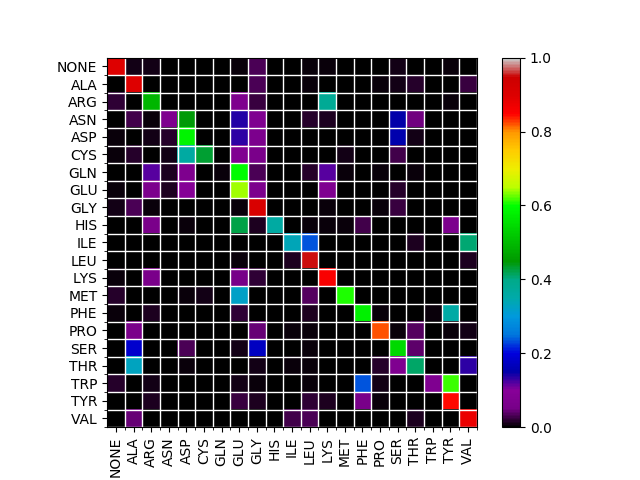
\includegraphics[width=1.27\textwidth]{pics/CM_22_SS}
	\caption{Confusion Matrix}
	\label{f:CM_22_SS}
\end{subfigure}
\end{minipage}
\begin{minipage}[b]{0.45\linewidth}
\begin{subfigure}[b]{\linewidth}
	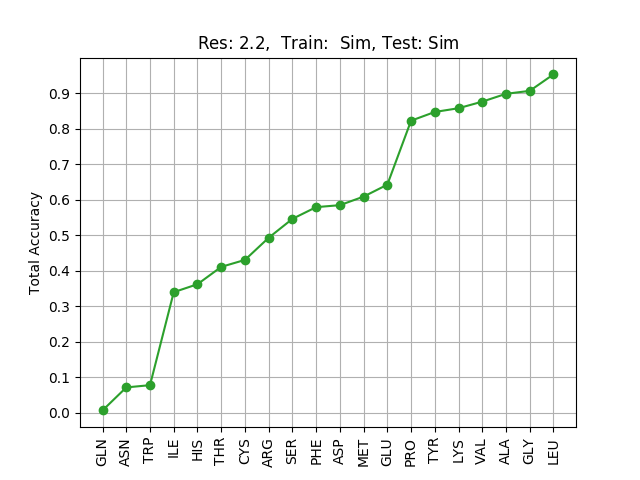
\includegraphics[width=1.27\textwidth]{pics/ss22_acc.png}
	\caption{Total Accuracy}
	\label{f:ss22_acc}
\end{subfigure}
\end{minipage}
\caption{Classification Results: Resolution $2.2 \AA$,  Train: Simulated, Test : Simulated}
\end{figure}

\begin{figure}[!ht]
\begin{minipage}[b]{0.45\linewidth}
\begin{subfigure}[b]{\linewidth}
	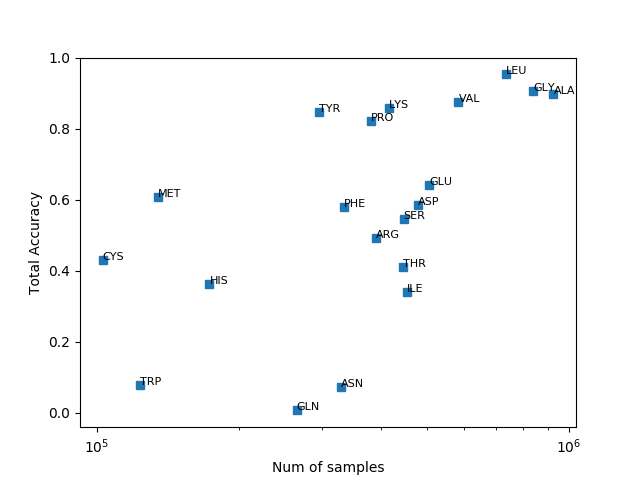
\includegraphics[width=1.1\textwidth]{pics/DS_22_SS}
	\caption{Accuracy vs Dataset size \newline \newline}
	\label{f:DS_22_SS}
\end{subfigure}
\end{minipage}
\begin{minipage}[b]{0.45\linewidth}
\begin{subfigure}[b]{\linewidth}
	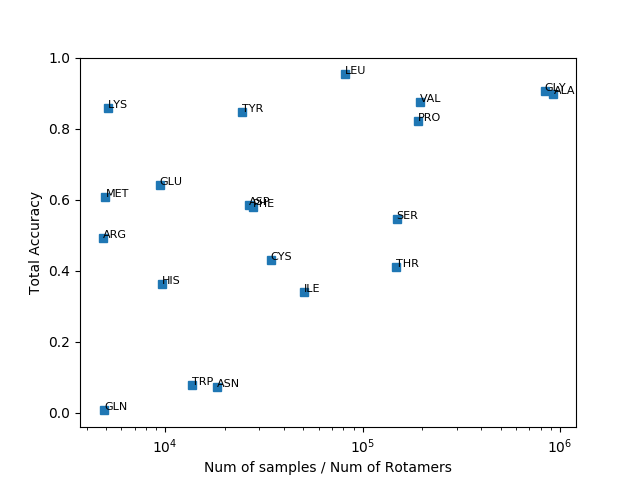
\includegraphics[width=1.1\textwidth]{pics/DS_norm_22_SS.png}
	\caption{Accuracy vs Dataset size normalized to the number of Rotamers}
	\label{f:DS_norm_22_SS}
\end{subfigure}
\end{minipage}
\caption{Effect of the Training Dataset Size on the Classification Accuracy: Resolution $2.2 \AA$,  Train: Simulated, Test : Simulated}
\end{figure}


\paragraph{Experimental Data Results}
We used a $2.2$ cryo-EM map of $\beta$-galactosidase (\cite[]{Bartesaghi2015}. EMD-2984) to study the CNN performance.
At the time of the research, only three additional cryoEM maps with resolution better than $2.3 \AA$ were available: EMD-8762 \cite[]{Dong2017}, EMD-8194 \cite[]{Merk2016}, and EMD-3295 \cite[]{Banerjee2016}.
Even augmented , this is definitely not enough for proper training of the CNN.
The confusion matrix and the total accuracies are shown in Figures ~\ref{f:CM_22_RR} and ~\ref{f:rr22_acc}.
The accuracy dependence on the dataset size is shown in Figures ~\ref{f:DS_22_RR} and ~\ref{f:DS_norm_22_RR}.
Despite significantly lower accuracies, the tendency observed on simulated data is preserved.

In order to improve the classification accuracy we tried two methods to overcome the lack of data:
\begin{enumerate}
\item We trained up to 6 independent CNNs and averaged the obtained probabilities.
\item We combined the real maps with the simulated maps and created  a new dataset.
\end{enumerate}
The first method, averaging over multiple networks, did not result in any significant improvement of the classification accuracy.
This indicates that the obtained low accuracy is not due to overfitting, but due to the small training set.
Best classification results were achieved by combining in the training set simulated and experimental data in equal proportion.
We denote the CNN trained on this combined dataset as $N^{22}_{ES}$.
The detection accuracies for this case are shown in Figures ~\ref{f:CM_22_RSR} and ~\ref{f:rsr22_acc}.

Figure ~\ref{f:rl_22} shows the estimated reliability curves for $N^{22}_{ES}$. 
Due to lack of data, reliability curves cannot be estimated for every input, but the overall tendency is that the output of the softmax layer of $N^{22}_{ES}$ underestimated the classification accuracy.

\begin{figure}[!ht]
\begin{minipage}[b]{0.45\linewidth}
\begin{subfigure}[b]{\linewidth}
	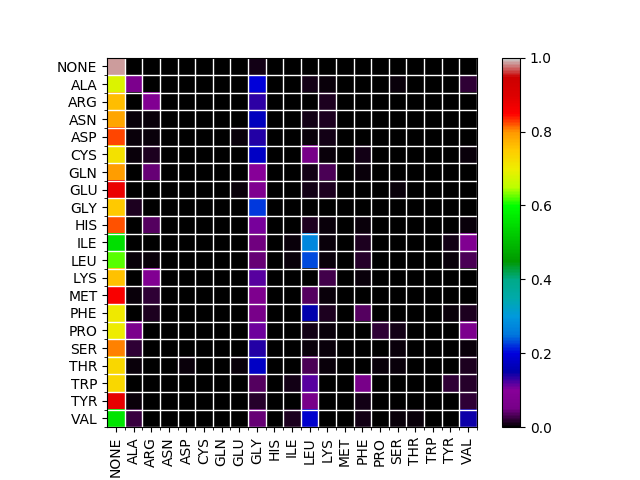
\includegraphics[width=1.27\textwidth]{pics/CM_22_RR}
	\caption{Confusion Matrix}
	\label{f:CM_22_RR}
\end{subfigure}
\end{minipage}
\begin{minipage}[b]{0.45\linewidth}
\begin{subfigure}[b]{\linewidth}
	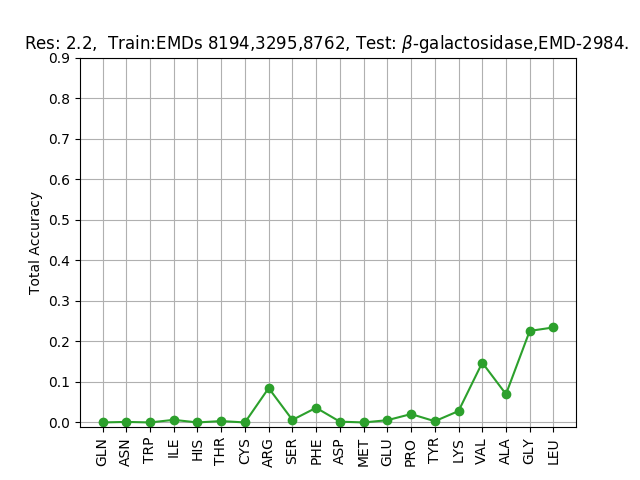
\includegraphics[width=1.27\textwidth]{pics/rr22_acc.png}
	\caption{Total Accuracy}
	\label{f:rr22_acc}
\end{subfigure}
\end{minipage}
\caption{Classification Results: Resolution $2.2 \AA$,  Train: EMDs 8762,3295,8184, Test : $\beta$-galactosidase, \cite[]{Bartesaghi2015}. }
\end{figure}

\begin{figure}[!ht]
\begin{minipage}[b]{0.45\linewidth}
\begin{subfigure}[b]{\linewidth}
	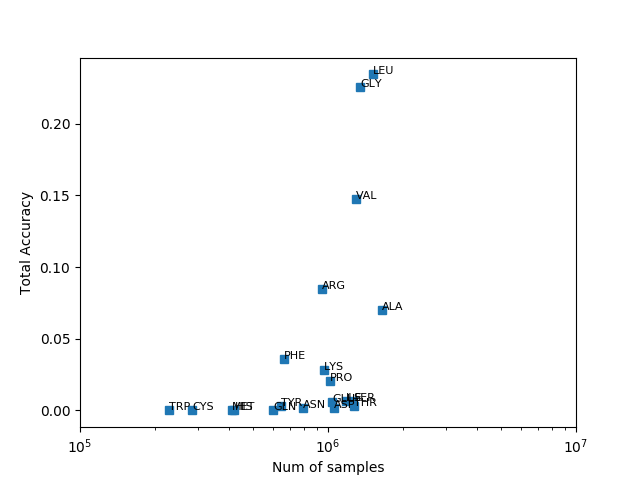
\includegraphics[width=1.1\textwidth]{pics/DS_22_RR}
	\caption{Accuracy vs Dataset size \newline \newline}
	\label{f:DS_22_RR}
\end{subfigure}
\end{minipage}
\begin{minipage}[b]{0.45\linewidth}
\begin{subfigure}[b]{\linewidth}
	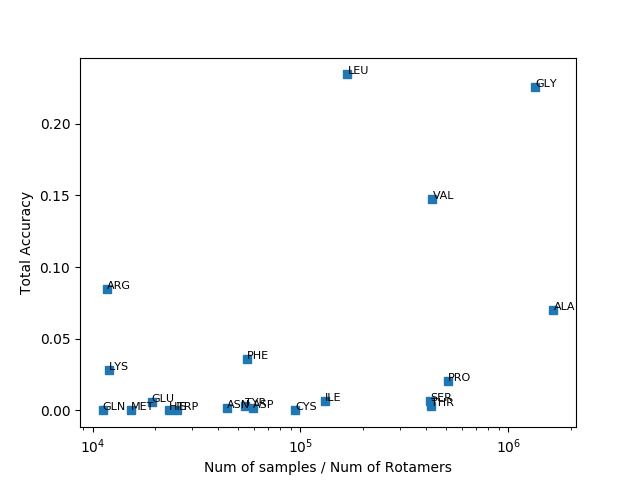
\includegraphics[width=1.1\textwidth]{pics/DS_norm_22_RR.png}
	\caption{Accuracy vs Dataset size normalized to a number of Rotamers}
	\label{f:DS_norm_22_RR}
\end{subfigure}
\end{minipage}
\caption{Effect of Training Dataset Size on the Classification Accuracy: Train: EMDs 8762,3295,8184, Test : $\beta$-galactosidase, \cite[]{Bartesaghi2015}.}
\end{figure}


\begin{figure}[!ht]
\begin{minipage}[b]{0.45\linewidth}
\begin{subfigure}[b]{\linewidth}
	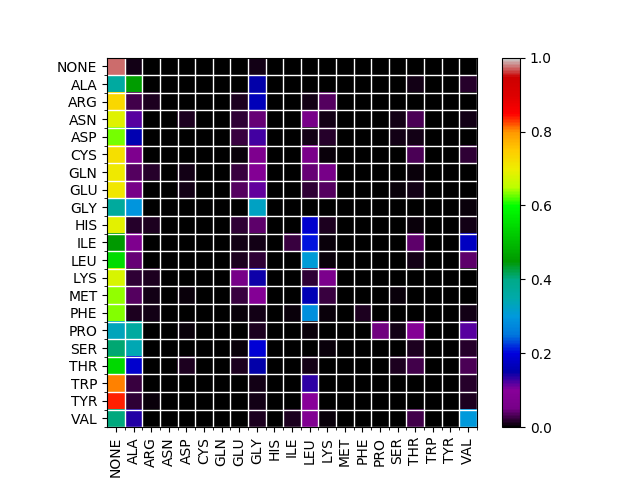
\includegraphics[width=1.27\textwidth]{pics/CM_22_RSR}
	\caption{Confusion Matrix}
	\label{f:CM_22_RSR}
\end{subfigure}
\end{minipage}
\begin{minipage}[b]{0.45\linewidth}
\begin{subfigure}[b]{\linewidth}
	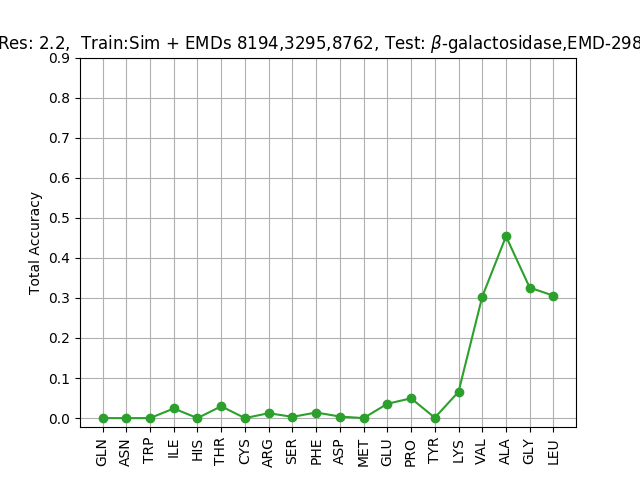
\includegraphics[width=1.27\textwidth]{pics/rsr22_acc.png}
	\caption{Total Accuracy}
	\label{f:rsr22_acc}
\end{subfigure}
\end{minipage}
\caption{Classification Results: Resolution $2.2 \AA$,  Train: Simulation + EMDs 8762,3295,8184, Test : $\beta$-galactosidase, \cite[]{Bartesaghi2015}. }
\end{figure}

\begin{figure}[!ht]
\begin{minipage}[b]{0.45\linewidth}
\begin{subfigure}[b]{\linewidth}
	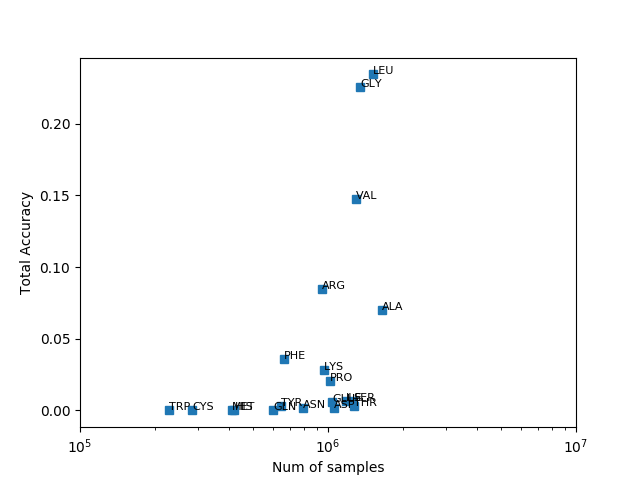
\includegraphics[width=1.1\textwidth]{pics/DS_22_RR}
	\caption{Accuracy vs Dataset size \newline \newline}
	\label{f:DS_22_RR}
\end{subfigure}
\end{minipage}
\begin{minipage}[b]{0.45\linewidth}
\begin{subfigure}[b]{\linewidth}
	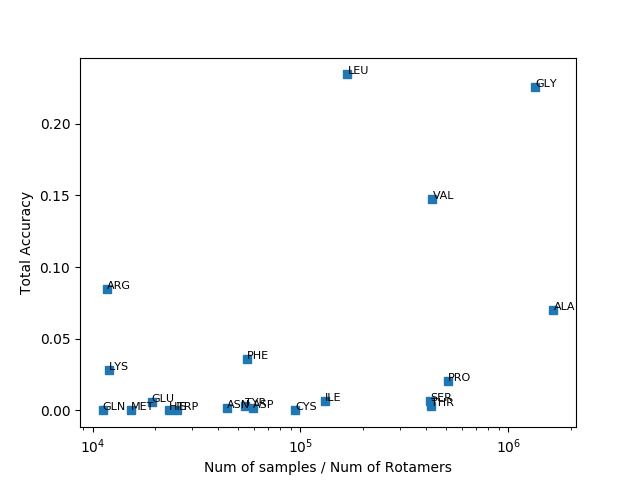
\includegraphics[width=1.1\textwidth]{pics/DS_norm_22_RR.png}
	\caption{Accuracy vs Dataset size normalized to the number of Rotamers}
	\label{f:DS_norm_22_RR}
\end{subfigure}
\end{minipage}
\caption{Effect of Training Dataset Size on the Classification Accuracy: Train: EMDs 8762,3295,8184, Test : $\beta$-galactosidase, \cite[]{Bartesaghi2015}.}
\end{figure}


\begin{figure}[!ht]
\begin{minipage}[b]{0.45\linewidth}
\begin{subfigure}[b]{\linewidth}
	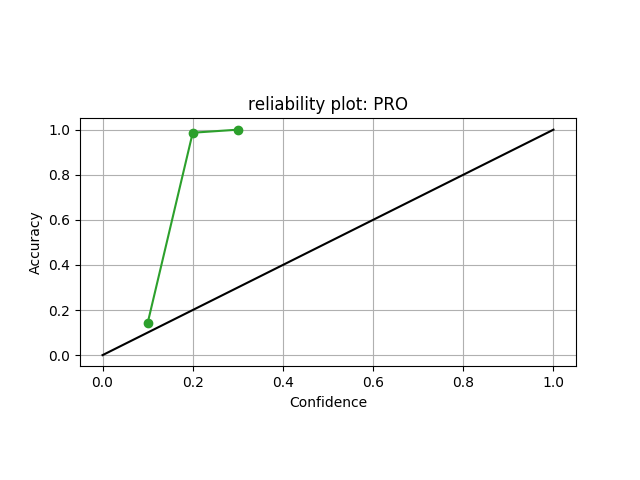
\includegraphics[width=1.27\textwidth]{pics/rel_PRO_22_SRS}
\end{subfigure}
\begin{subfigure}[b]{\linewidth}
	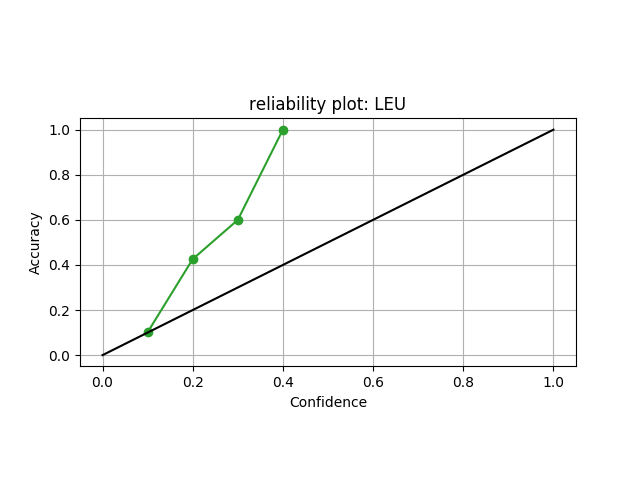
\includegraphics[width=1.27\textwidth]{pics/rel_LEU_22_SRS}
\end{subfigure}

\end{minipage}
\begin{minipage}[b]{0.45\linewidth}
\begin{subfigure}[b]{\linewidth}
	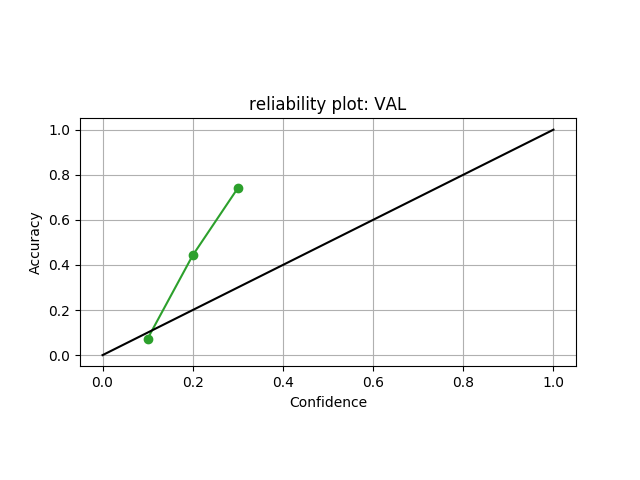
\includegraphics[width=1.27\textwidth]{pics/rel_VAL_22_SRS}
\end{subfigure}
\begin{subfigure}[b]{\linewidth}
	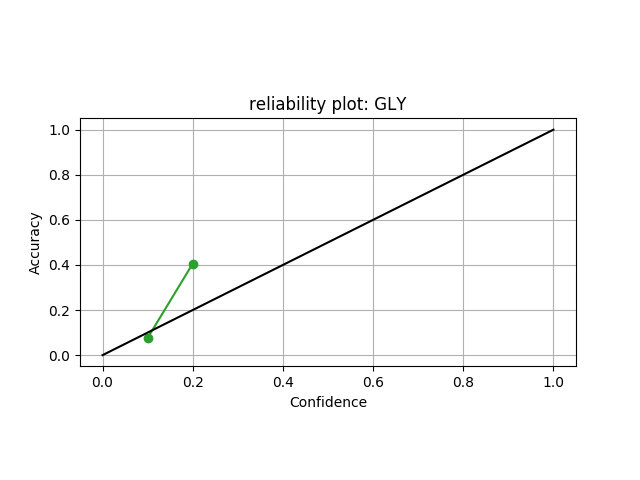
\includegraphics[width=1.27\textwidth]{pics/rel_GLY_22_SRS}
\end{subfigure}
\end{minipage}
\caption{Estimated Reliability Curves for PRO, LEU, VAL, GLY : Resolution $2.2 \AA$,  Train: Simulation + EMDs 8762,3295,8184, Test : $\beta$-galactosidase, \cite[]{Bartesaghi2015}. }\label{f:rl_22}
\end{figure}


\subsubsection{Resolutions $2.9 \AA$ and   $3.1 \AA$ }
Coarsening the resolution has two opposite effects on the classification accuracy.
Intuitively, in higher resolution maps the amino acids shape is sharper, but lower resolution maps benefit from a larger training dataset.
The size of the training dataset for three tested resolutions is shown on Table ~\ref{t0}.
The effect of a map resolution on the classification accuracy is shown in Figures ~\ref{f:s3_293_acc} and ~\ref{f:r3_293_acc}.
While having only a small effect on simulated data (Figure ~\ref{f:s3_293_acc}), the effect of resolution on the real data is well expressed (Figure ~\ref{f:r3_293_acc}).
 Accuracies for $2.9 \AA$ and $3.1 \AA$ are significantly better than those for $2.2 \AA$. This is clearly due to the increased training dataset. 
 The only exception is Alanin, which is probably too small to be detected at resolutions above $2.2 \AA$.
However, moving from $2.9 \AA$ to $3.1 \AA$ we see that for the majority of the amino acids the total accuracy values are decreased.  Thus, in this transition the effect of increasing the training dataset size did not compensate for the degradation in map precision.
 
The confusion matrices for $2.9 \AA$ Anthrax toxin protective antigen pore and $3.1 \AA $ Lysenin Pore are presented in Figures ~\ref{f:CM_29_RR} and ~\ref{f:CM_31_RR}, respectively. The Reliability Curves for the $2.9 \AA$ Anthrax toxin protective antigen pore and $3.1 \AA $ Lysenin Pore are presented in Figures ~\ref{f:CM_29_RR} ~\ref{f:CM_31_RR}, respectively.
 While at resolution of $2.9 \AA$ the estimated confidence is still less than the observed one, at $3.1 \AA$ resolution the estimated confidence is of good precision.
 
\begin{table}
\small
\begin{tabular}{ | m{5em} | m{1cm} | m{3cm}| }
\hline
 Resolution Span & N. Maps  & Map for Validation \\
\hline
 $1.8-2.3 \AA$  & 3  & EMD-2984 , $2.2 \AA$ $beta$ -galactosidase \cite[]{Banerjee2016} \\
\hline
 $2.7-2.9 \AA$  & 8  & EMD-6224 ,$2.9 \AA$  Anthrax toxin protective antigen pore \cite[]{Jiang2015} \\
\hline
 $2.9-3.1 \AA$  & 13  & EMD -8015, $3.1 \AA$ Lysenin Pore \cite[]{Bokori-Brown2016} \\
\hline
 \end{tabular}
\caption{Experimental Train and Test data for Various Resolutions}\label{t0}
\end{table}

\begin{figure}[!ht]
\begin{minipage}[b]{0.45\linewidth}
\begin{subfigure}[b]{\linewidth}
	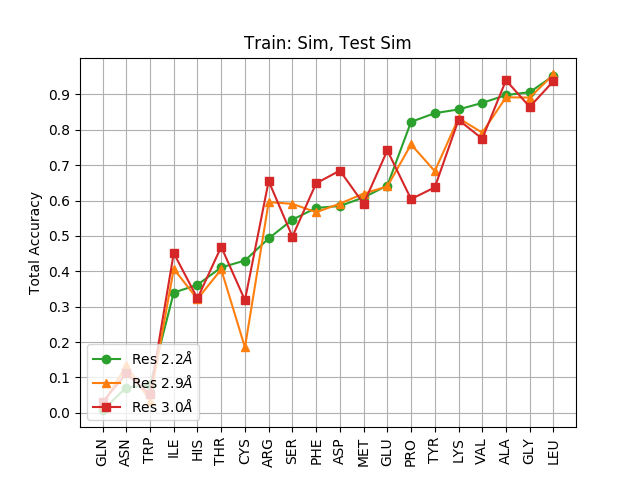
\includegraphics[width=1.1\textwidth]{pics/s3_293_acc}
	\caption{Simulated Data \newline \newline}
	\label{f:s3_293_acc}
\end{subfigure}
\end{minipage}
\begin{minipage}[b]{0.45\linewidth}
\begin{subfigure}[b]{\linewidth}
	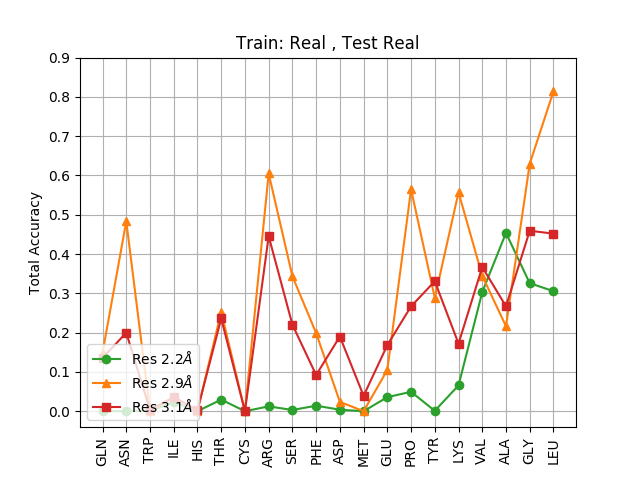
\includegraphics[width=1.1\textwidth]{pics/r3_293_acc}
	\caption{Real Data (Mixed with Simulation for Resolution $2.2 \AA$}
	\label{f:r3_293_acc}
\end{subfigure}
\end{minipage}
\caption{Total classification accuracies for different resolutions.}
\end{figure}


\begin{figure}[!ht]
\begin{minipage}[b]{0.45\linewidth}
\begin{subfigure}[b]{\linewidth}
	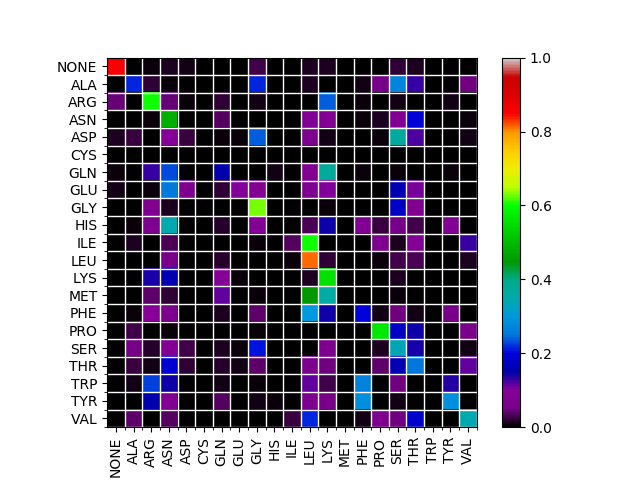
\includegraphics[width=1.2\textwidth]{pics/CM_29_RR}
	\caption{Accuracy vs Dataset size \newline \newline}
	\label{f:CM_29_RR}
\end{subfigure}
\end{minipage}
\begin{minipage}[b]{0.45\linewidth}
\begin{subfigure}[b]{\linewidth}
	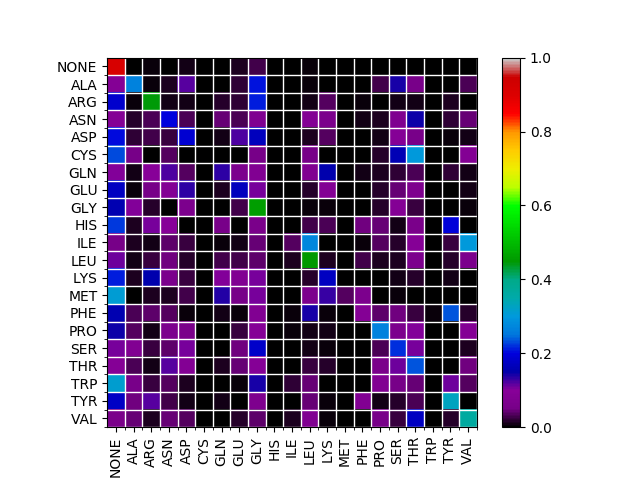
\includegraphics[width=1.2\textwidth]{pics/CM_31_RR.png}
	\caption{Accuracy vs Dataset size normalized to a number of Rotamers}
	\label{f:CM_31_RR}
\end{subfigure}
\end{minipage}
\caption{Classification Accuracy Results for Resolution $2.9$ and $3.1$ }
\end{figure}

\begin{figure}[!ht]
\begin{minipage}[b]{0.45\linewidth}
\begin{subfigure}[b]{\linewidth}
	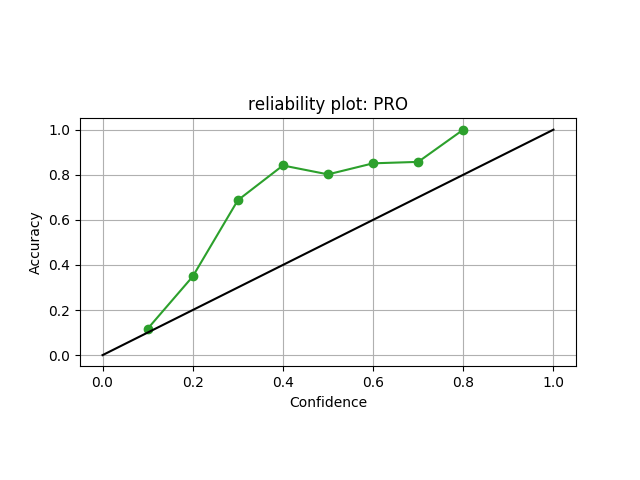
\includegraphics[width=1.27\textwidth]{pics/rel_PRO_29_RR}
\end{subfigure}
\begin{subfigure}[b]{\linewidth}
	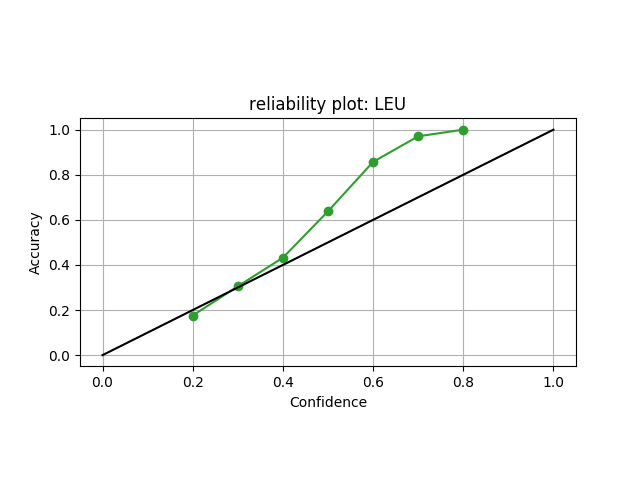
\includegraphics[width=1.27\textwidth]{pics/rel_LEU_29_RR}
\end{subfigure}

\end{minipage}
\begin{minipage}[b]{0.45\linewidth}
\begin{subfigure}[b]{\linewidth}
	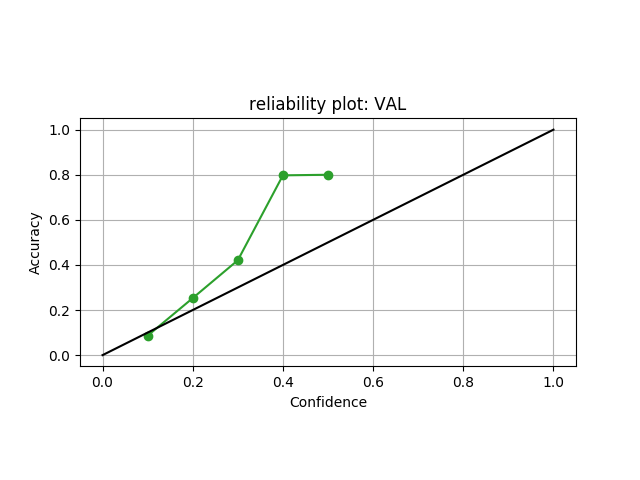
\includegraphics[width=1.27\textwidth]{pics/rel_VAL_29_RR}
\end{subfigure}
\begin{subfigure}[b]{\linewidth}
	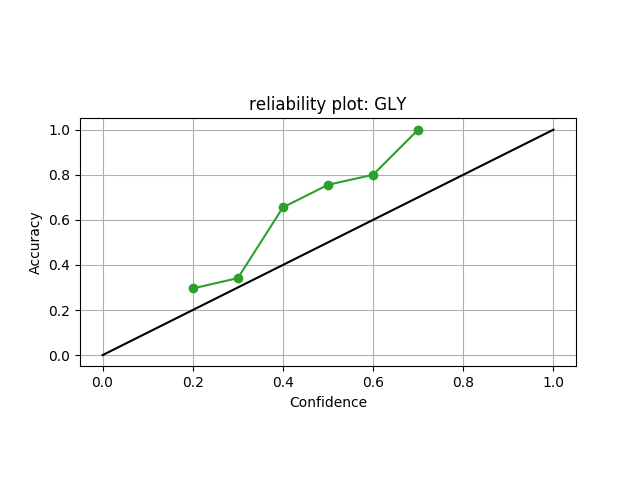
\includegraphics[width=1.27\textwidth]{pics/rel_GLY_29_RR}
\end{subfigure}
\end{minipage}
\caption{Estimated Reliability Curves for PRO, LEU, VAL, GLY : Resolution $2.9 \AA$,  Train: Experimental Data, Test :  Anthrax toxin protective antigen pore \cite[]{Jiang2015}.}\label{f:rl_29}
\end{figure}

\begin{figure}[!ht]
\begin{minipage}[b]{0.45\linewidth}
\begin{subfigure}[b]{\linewidth}
	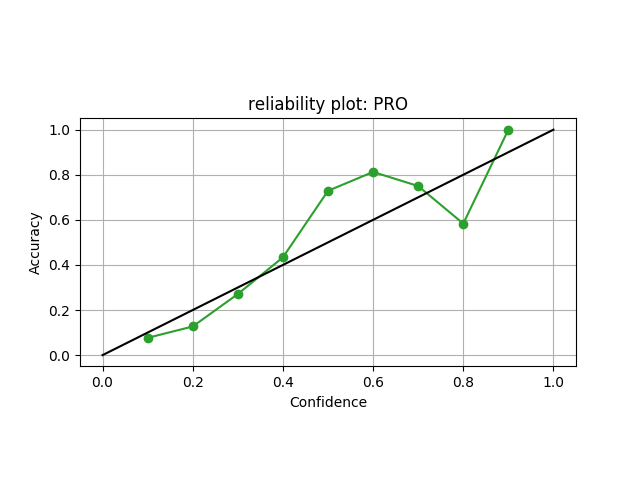
\includegraphics[width=1.27\textwidth]{pics/rel_PRO_31_RR}
\end{subfigure}
\begin{subfigure}[b]{\linewidth}
	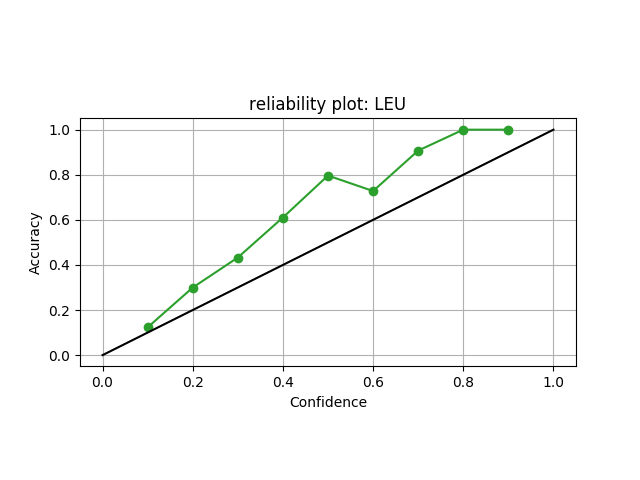
\includegraphics[width=1.27\textwidth]{pics/rel_LEU_31_RR}
\end{subfigure}

\end{minipage}
\begin{minipage}[b]{0.45\linewidth}
\begin{subfigure}[b]{\linewidth}
	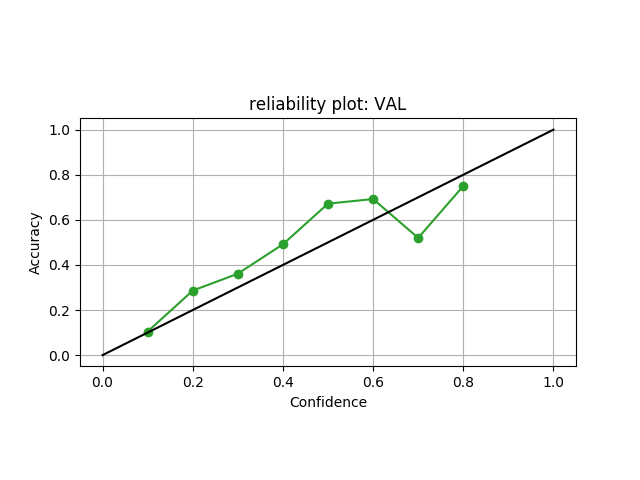
\includegraphics[width=1.27\textwidth]{pics/rel_VAL_31_RR}
\end{subfigure}
\begin{subfigure}[b]{\linewidth}
	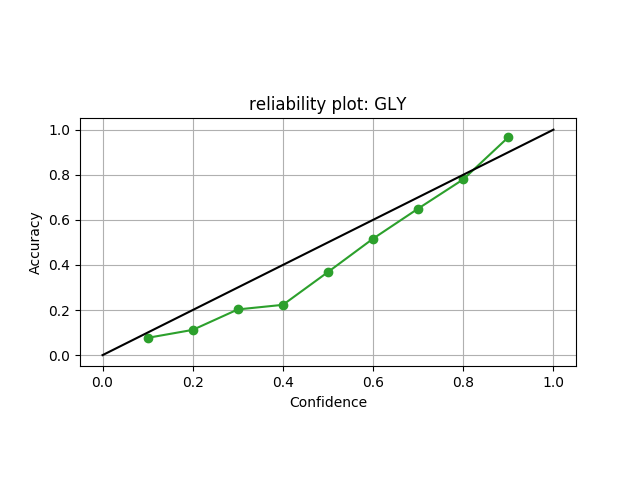
\includegraphics[width=1.27\textwidth]{pics/rel_GLY_31_RR}
\end{subfigure}
\end{minipage}
\caption{Estimated Reliability Curves for PRO, LEU, VAL, GLY : Resolution $3.1 \AA$,  Train: Experimental Data, Test :  Lysenin Pore \cite[]{Bokori-Brown2016}. }\label{f:rl_31}
\end{figure}


\subsection{Detection Results}
In the detection (also called localization) task, the exact location of an amino acid is unknown. 
Whilst the localization of all amino acids of a protein seems to be a hard problem at this time, detection of a subset of the amino acids obtained with high confidence is achievable. 
In this paper we focused on identifying \textbf{anchors}, i.e., amino acids, which have been located and labeled with confidence above $80 \%$. 


For each resolution case we tested a number of different classification methods, while the pre-processing and post-processing phases remain unchanged.

Table ~\ref{t22} summarizes the detection picks for the $2.2\AA$ map of $beta$-galactosidase \cite[]{Bartesaghi2015}.  
There we succeed to detect amino acids of four types: ARG, LEU, PRO, VAL with confidence above $80\%$.
The fraction of the detected high confidence amino acids is up to $10 \%$ from the total amount of the same type.
We expect this result to improve, as more high resolution cryo EM maps are being released.


Table \ref{t29} summarizes the detection picks for the test map of the $2.9\; \AA$ resolution anthrax toxin protective antigen pore \cite[]{Jiang2015}.  
We succeded to detect $70 \%$ of the Prolines.
Figure ~\ref{f:PRO29} illustrates the results of proline detection.
The detection rate of ARG, LEU, TYR,VAL was about $20 \%$.

Table \ref{t31} summarizes the detection picks for the test map of $3.1 \; \AA$ resolution Lysenin Pore \cite[]{Bokori-Brown2016}.
We detected more than $20 \%$ of the Leucine residues.
We also succeded to detect about $10 \%$ of LYS, TYR, ARG, GLY and PRO.
Figure ~\ref{f:LYS31} illustrates the detection results for LEU, LYS, TYR and GLY at map resolution of $3.1 \AA$.

Note that the use of simulated data was crucial for the $2.2 \AA$ resolution experiment.
For resolutions $2.9 \AA$ and   $3.1 \AA$ the role of simulated data is less important, since more experimental maps are available.

\begin{table}
\small
\begin{tabular}{ | m{4em} | m{1.5cm} || m{1.5cm}|| m{2.6cm}| } 
 \hline
 Amino Acid Type & Picks with Confidence of $80\%$   & Total in Protein & Best Method \\
 \hline
\hline
ARG  & 17  & 133 & $maj(N_S,N_E,N_{ES})$  \\
\hline
LEU  & 15    & 231 & $mean(N_S,N_E,N_{ES})$   \\
\hline
PRO  & 10    & 189 & $N_{ES}$  \\
\hline
VAL  & 10    & 119 & $mean(N_S,N_E,N_{ES})$  \\
\hline
\end{tabular}
\caption{Detection Results $2.2 \; \AA$ cryo-EM single particle reconstruction of beta galactosidase (emd-2984)}\label{t22}
\end{table}


\begin{table}
\begin{tabular}{ | m{4em} | m{1.5cm} || m{1.5cm}|| m{2.6cm}| } 
 \hline
 Amino Acid Type & Picks with Confidence of $80\%$  & Total in Protein & Best Method \\
 \hline
\hline
ASN  & 5    & 287 & $N_E$  \\
\hline
ARG  & 20    & 119 & $N_E$  \\
\hline
LEU  & 40    & 231 & $N_E$  \\
\hline
LYS  & 30    & 189 & $mean(N_S,N_E)$  \\
\hline
PRO  & 80  & 133 & $maj(N_S,N_E,N_{ES})$  \\
\hline
TYR  & 18    & 91 & $N_{ES}$  \\
\hline
VAL  & 35    & 161 & $N_E$  \\
\hline
\end{tabular}
\caption{Detection results for $2.9 \; \AA$ CryoEM single particle reconstruction of an "anthrax toxin protective antigen pore (emd-6224)"}\label{t29}
\end{table}
\begin{table}
\begin{tabular}{ | m{4em} | m{1.5cm} || m{1.5cm}|| m{2.6cm}| } 
 \hline
 Amino Acid Type & Picks with Confidence of $80\%$  & Total in Protein & Best Method \\
 \hline
\hline
ARG  & 10  & 117 & $N_{ES}$  \\
\hline
GLY  & 25  & 207 & $N_E$  \\
\hline
LEU  & 25  & 108 & $N_E$  \\
\hline
LYS  & 20  & 171 & $N_E$  \\
\hline
PRO  & 9  & 72 & $mean(N_R,N_E)$  \\
\hline
TYR  & 18  & 144 & $maj(N_R,N_E,N_{ES})$  \\
\hline

\end{tabular}
\caption{Detection results for $3.1 \; \AA$ CryoEM single particle reconstruction of an "Lysenin Pore (emd-8015)"}\label{t31}
\end{table}

\begin{figure}[!ht]
  \caption{Proline detection in  $2.9 \; \AA$ CryoEM single particle reconstruction of an "anthrax toxin protective antigen pore (emd-6224). Purple regions indicate the detected proline residues} \label{f:PRO29}
  \centering
    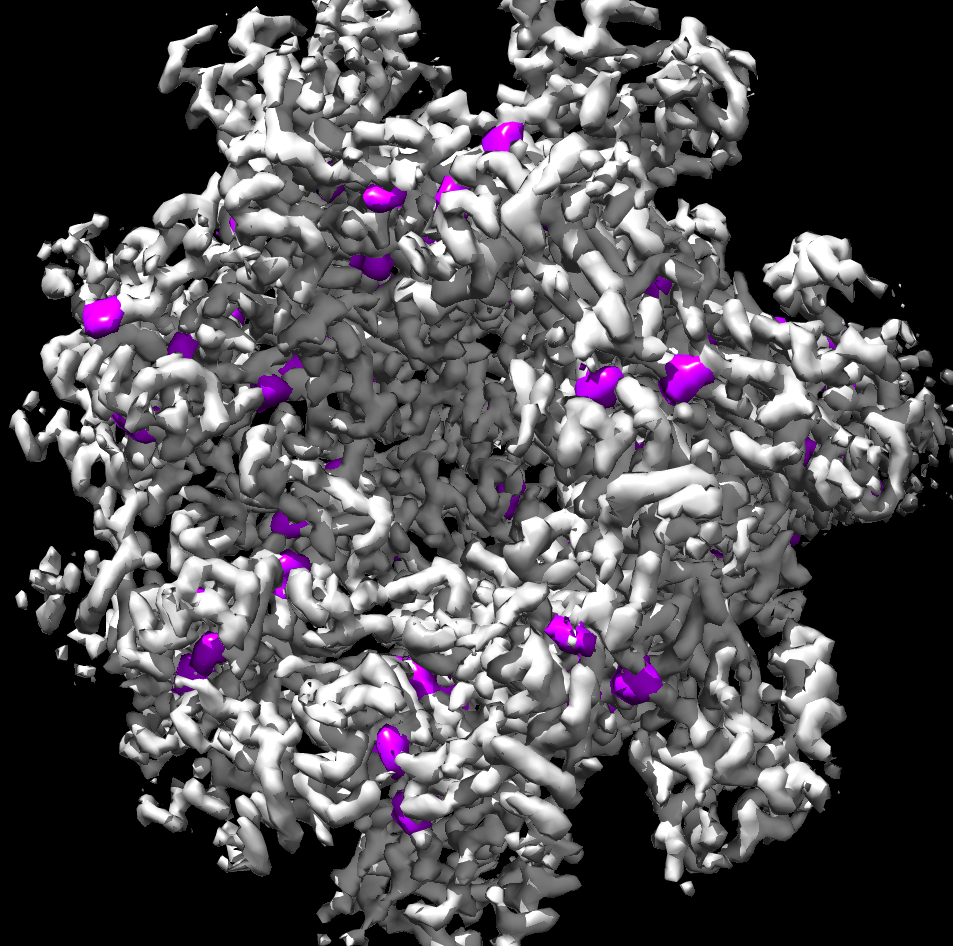
\includegraphics[width=0.5\textwidth]{pics/map_PRO.png}
\end{figure}

\begin{figure}[!ht]
  \caption{Detection leucines, lysines, glycines and tyrosines  in  $3.1 \; \AA$ CryoEM single particle reconstruction of single particle reconstruction of an "Lysenin Pore (emd-8015)". Red regions indicate the detected {\color{red} leucines}, blue regions indicate the detected {\color{blue} lysines}, yellow regions indicate the detected {\color{yellow} glycines}, and green regions indicate the detected {\color{green} tyrosines} } \label{f:LYS31}
  \centering
    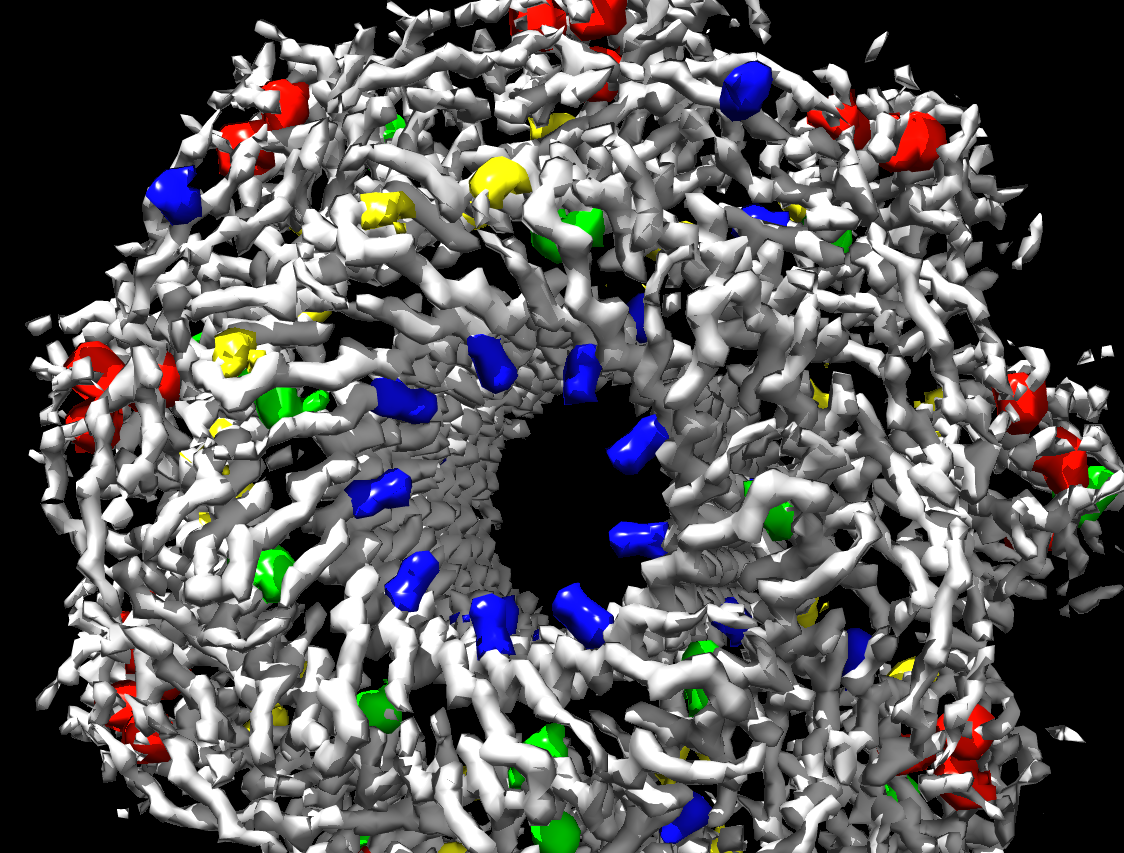
\includegraphics[width=0.5\textwidth]{pics/lys_pore_GLY_LEU_LYS_TYR.png}
\end{figure}

% Denote by 
% For our analysis we use the following quantities:
% \begin{itemize}
% 	\item \textbf{Recall} or hit rate (also true positive rate) for a label $j$ defined as $R(j) = \frac{T_j^j}{N_j}$
%     \item text
% \end{itemize}



% \subsection{Detection}
% \subsubsection{Resolution 2.2 Detection Results}
% \subsection{Precision- Recall curves}
% Precision (P) is defined as the number of true positives ($T_p$) over the number of true positives plus the number of false positives ($F_p$).
% $$
% P = \frac{T_p}{T_p+F_p}
% $$

% Recall ($R$) is defined as the number of true positives ($T_p$) over the number of true positives plus the number of false negatives ($F_n$).

% $$ R = \frac{T_p}{T_p + F_n} $$
\section{Web server Implementation}
We have developed a server of the detection/prediction stage of the  AAnchor algorithm at \url{http://bioinfo3d.cs.tau.ac.il/AAnchor/}.
The server outputs the detection results in PDB format, so that they could be displayed in commonly used programs such as UCSF Chimera \cite{Pettersen2004UCSFAnalysis}.
Figure ~\ref{f:t2} illustrates the server output as shown in UCSF Chimera.
Yellow spheres, which mark the predicted locations of prolines, are superimposed with 
the reference atomic model. 
\begin{figure}
  \caption{Detection of proline residues in a $ 2.9 \; \AA$ Cryo EM map. Yellow spheres show the predicted centers of mass for each of the detected amino acids. } \label{f:t2}
  \centering
    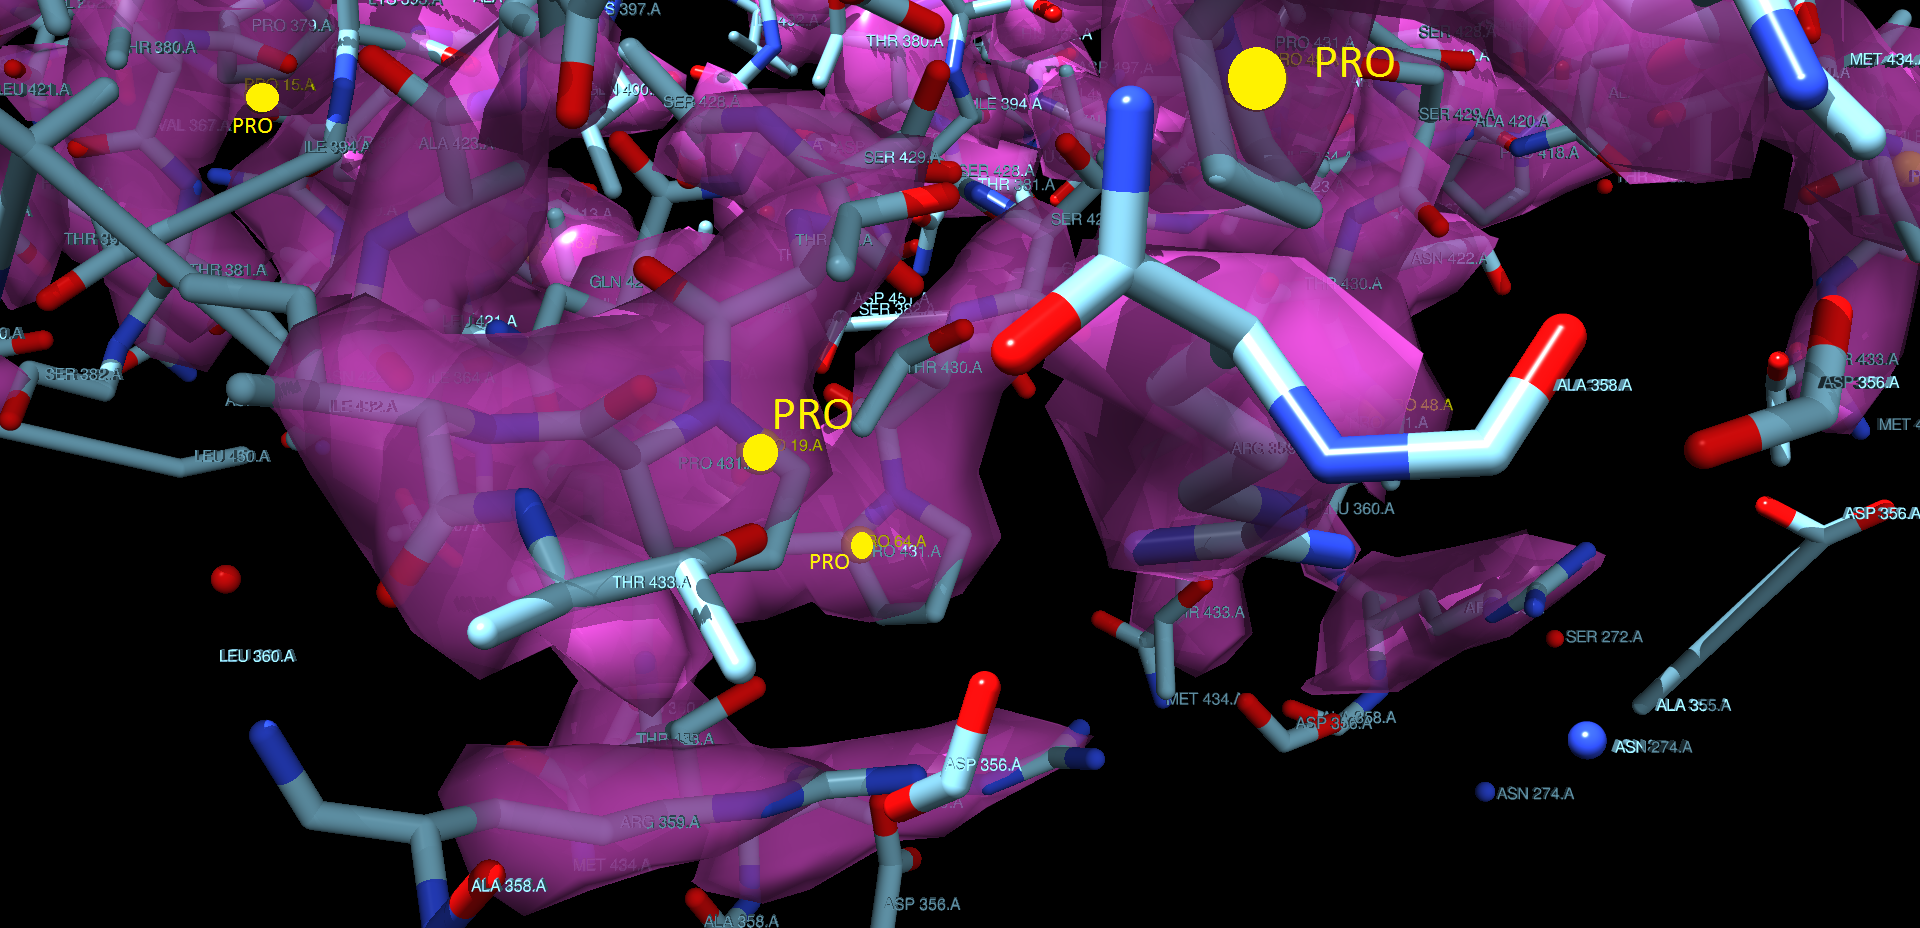
\includegraphics[width=0.5\textwidth]{pics/t2.png}
\end{figure}

\section{Conclusions}
In this paper we present a CNN based method for localization and classification of amino acids in high resolution cryo EM maps.
Whilst the \textit{de-novo} detection of all protein residues is still a hard problem, we succeeded to detect with high confidence a significant percentage of some amino acids.  
Experimental results show that the proposed method is capable of detecting a sufficient number of amino acid "anchors" in a cryo Em map of resolution $3.1 \AA$ or higher.
The reported confidence of a detection is at least as the ground truth accuracy.  These anchors can be further exploited in conjunction with several proposed modeling techniques as well as in the development of novel modeling methods.

We analyzed the detection process and factors affecting the classification task and concluded
that the number of rotamers for a given residue and the size of the training data set have a dominant effect on  the  detection rate, while the amino acid size plays a secondary role.
Contrary to expectation, the results for $2.9-3.1 \;\AA$ resolution maps have a  better detection potential than the more accurate $2.2 \;\AA$ maps. This is due to the limited training data set existing for the better resolution samples.
Also the detection accuracy  can be significantly improved by combining simulated and experimental cryo EM maps to compensate for the lack of experimental data.

As the number of released high resolution maps grows \cite[]{Lawson2016}, the detection accuracy will rise. 
Applying post processing techniques such as Linear Regression \cite[]{Naseem2010} and SVM \cite[]{Girshick2014} may potentially decrease the number of false detections.
Hopefully, with the accumulation of a sufficiently large number of experimental maps the classification of all voxels in a map to the different amino acids will be solvable using the Fully Convolutional CNN \cite[]{Long2015} technique.

\bibliography{all_ref}{}
\bibliographystyle{agsm}


\end{document}
